\documentclass{article}

\usepackage[utf8]{inputenc}
\usepackage{graphicx}
\usepackage{url}
\usepackage{color}
\usepackage{titlesec}
\usepackage{amsmath}
\usepackage{physics}
\usepackage{amsfonts}
\graphicspath{{../figures/}}

\title{paper draft: supersat}
\author{K. Latimer}
\date{Jan 13, 2020}

\begin{document}

\maketitle


\section{Introduction}
introductory notes.
\section{Theory + Simulation}
\begin{itemize}
	\item brief statement of quasi steady state formula 
	\item we see agreement between actual and QSS supersaturation under the conditions (see figs \ref{wrfvsqssunpoll} and \ref{wrfvsqsspoll}):
	\begin{itemize}
		\item T \textgreater 273K (we're not including ice in the theory)
		\item w \textgreater 2 m/s (reasonably strong updrafts)
		\item cloud LWC \textgreater 1e-4 g/g (in the convection core)
	\end{itemize}
	\item upon applying above filters, the distributions of $SS_{QSS}$, $w$, and LWC (cloud only) are shown in figs \ref{wrfqsshist}, \ref{wrfwhist}, and \ref{wrflwchist}.
\end{itemize}
\begin{figure}[ht]
    \centering
    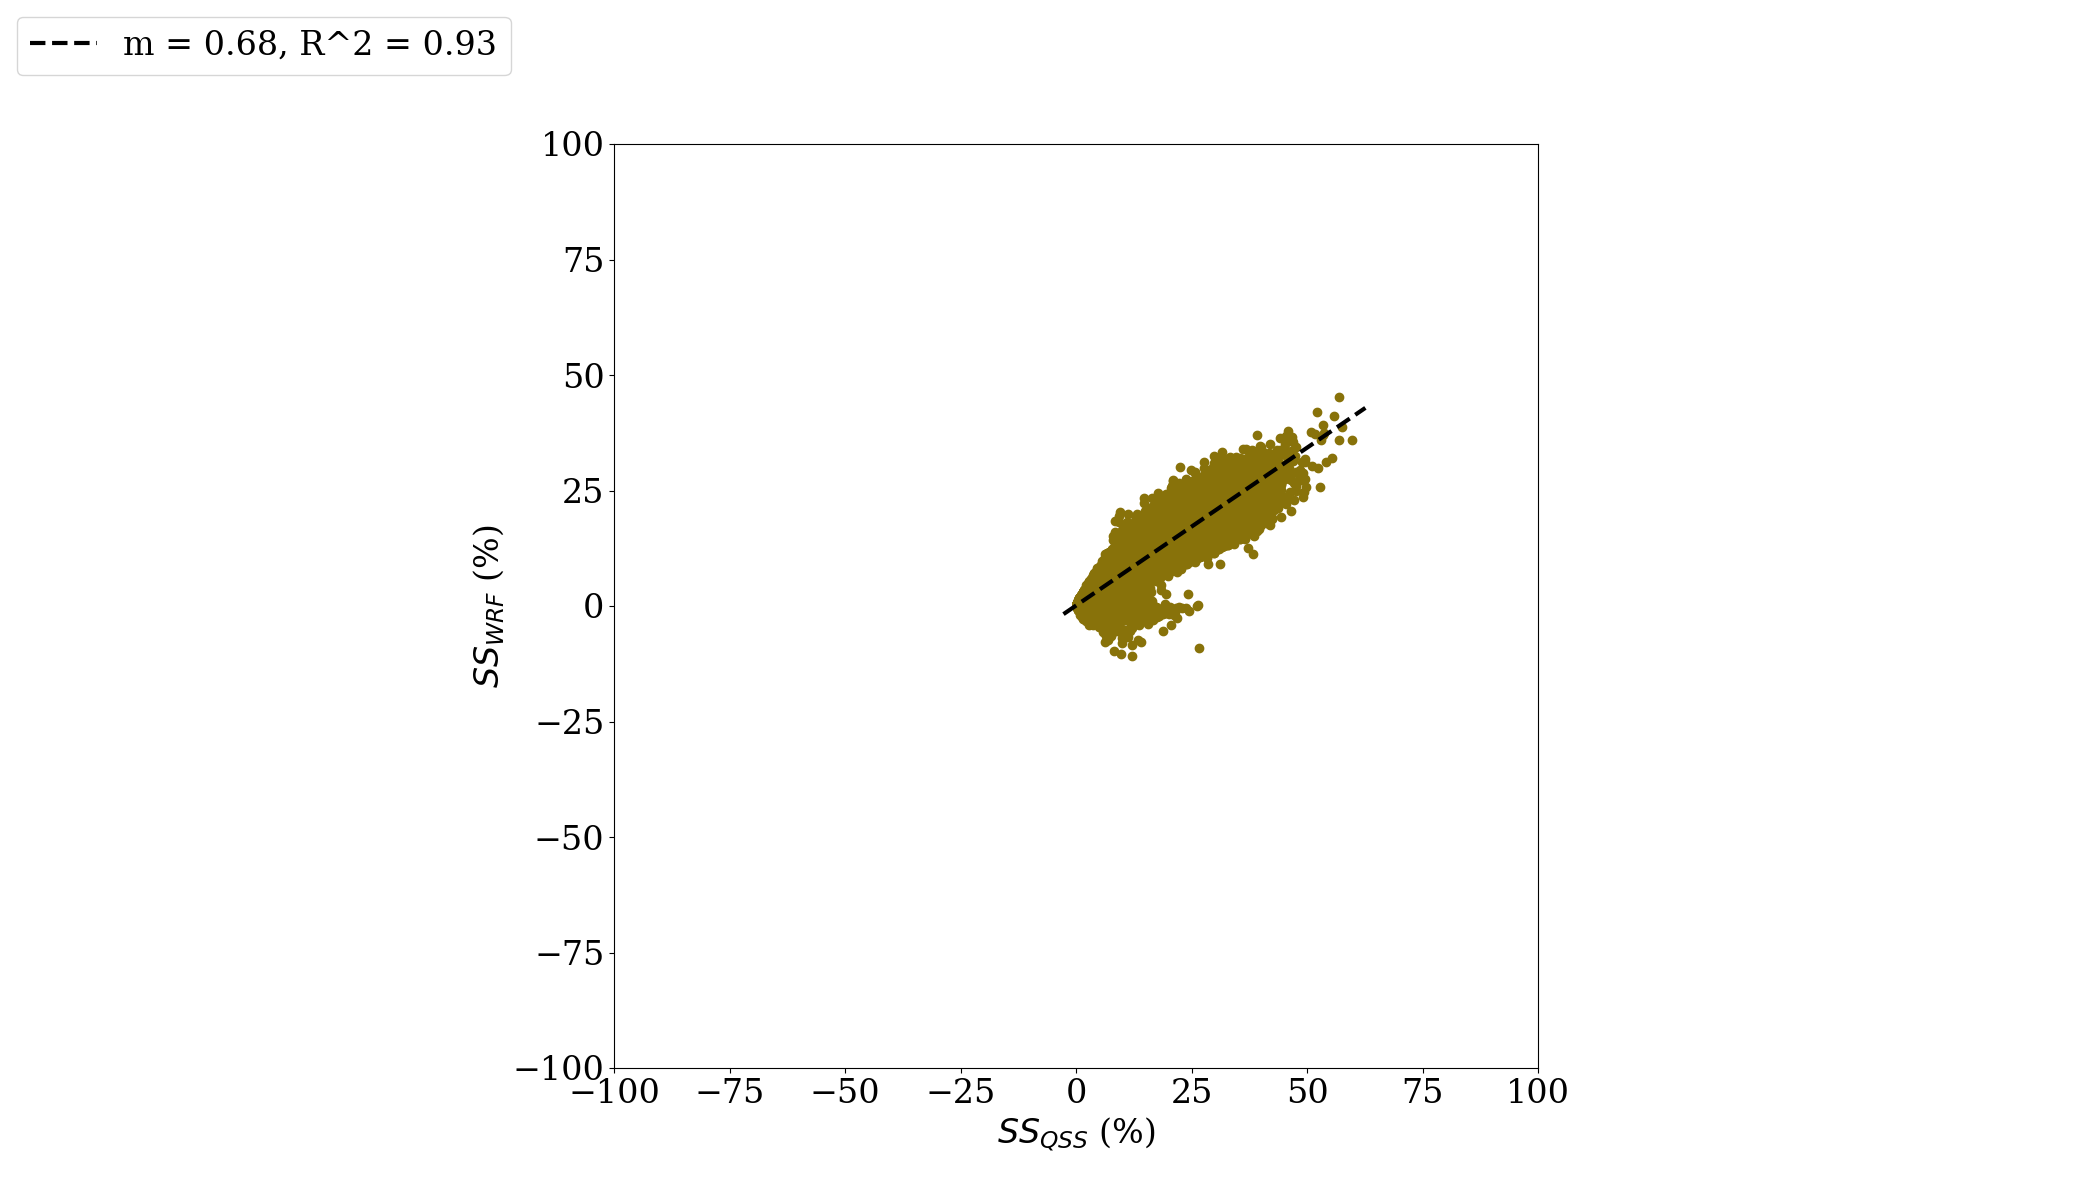
\includegraphics[width=9cm]{mywrf/v28_inclrain_and_vent_qss_vs_fan_Unpolluted_figure.png}
    \caption{Actual ($SS_{WRF}$) vs predicted ($SS_{QSS}$) supersaturation in unpolluted case.}
    \label{wrfvsqssunpoll}
\end{figure}
\begin{figure}[ht]
    \centering
    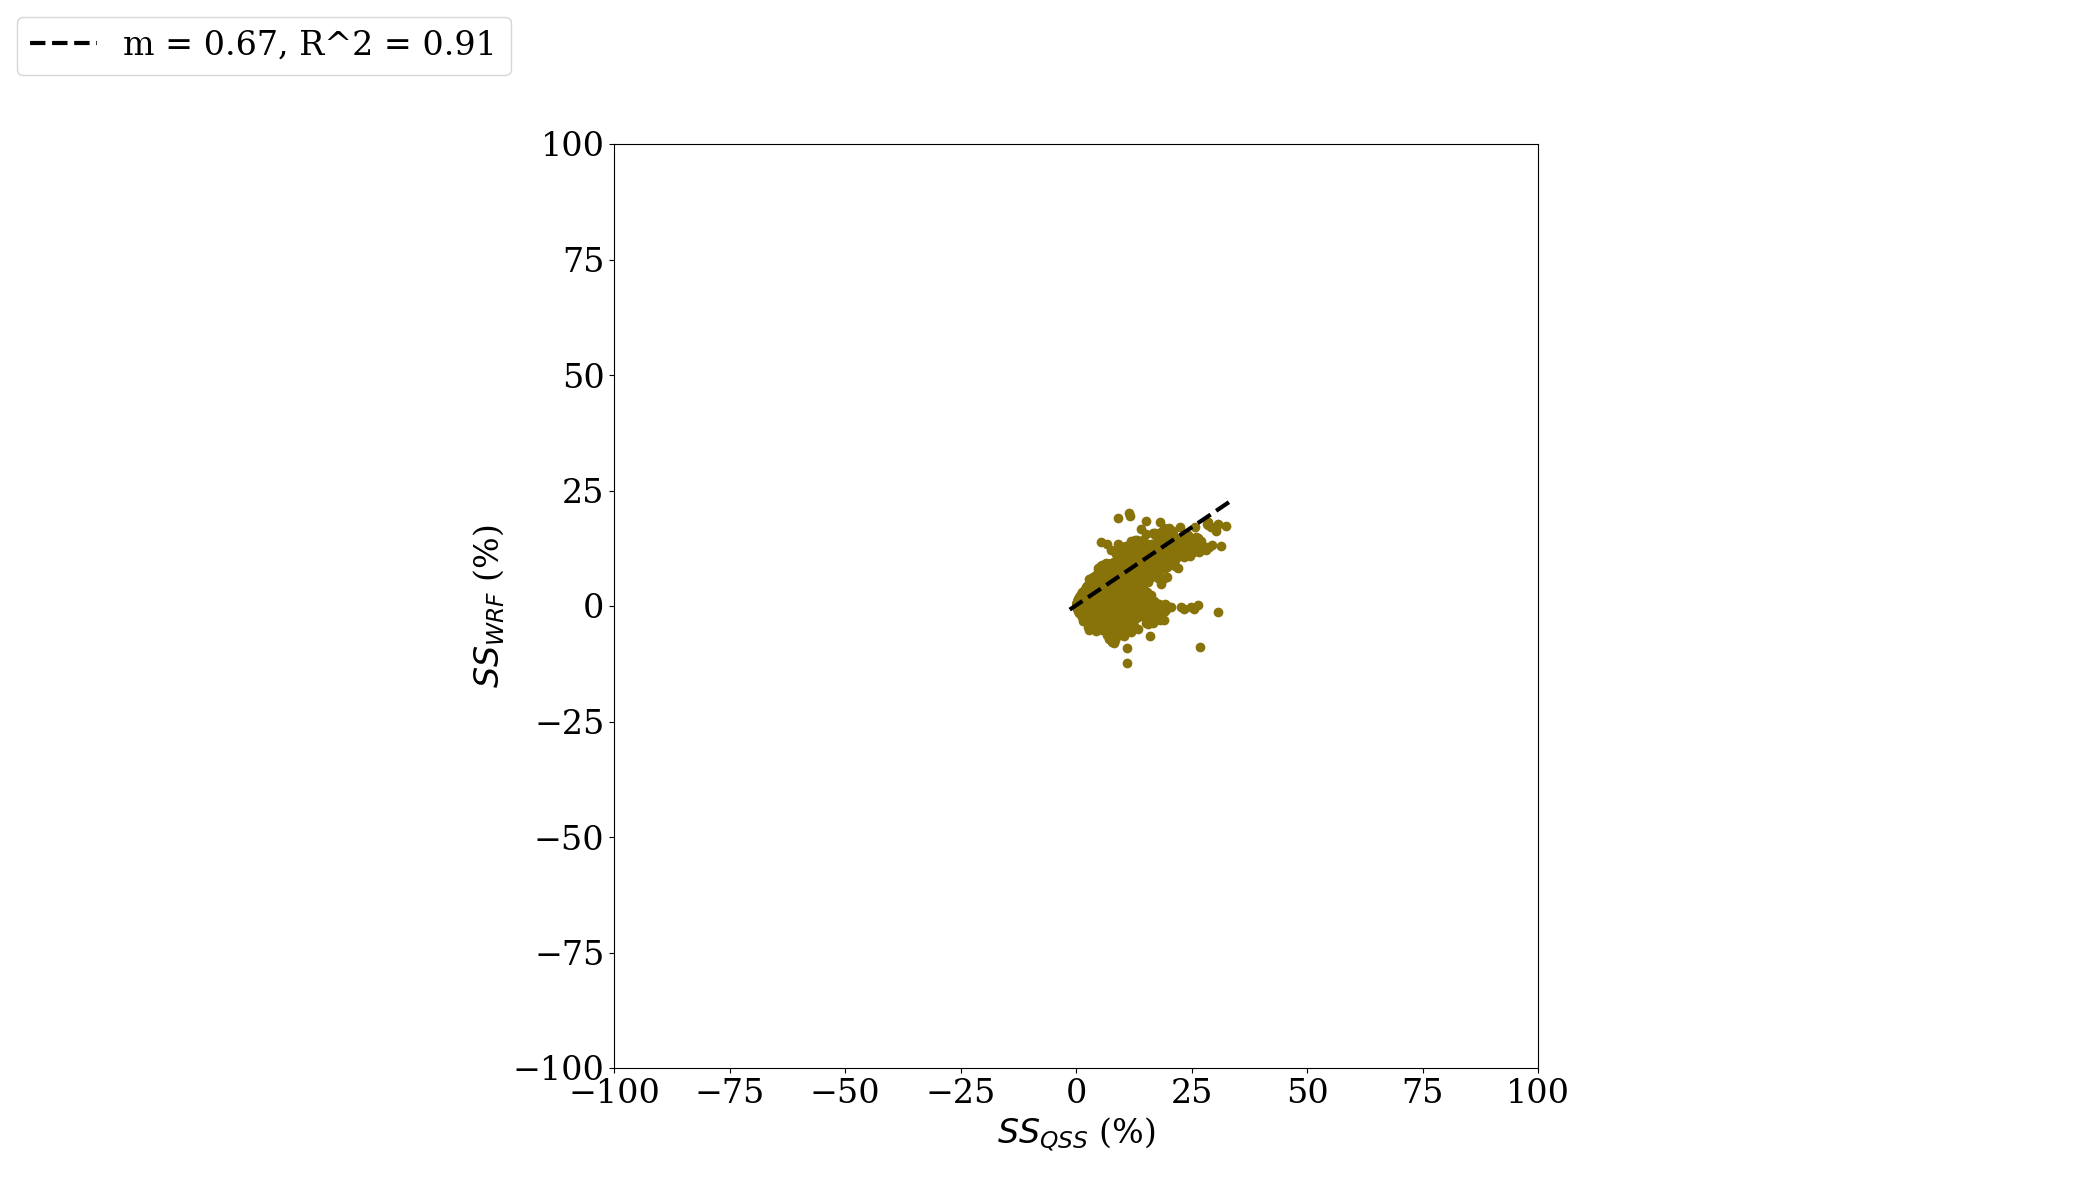
\includegraphics[width=9cm]{mywrf/v28_inclrain_and_vent_qss_vs_fan_Polluted_figure.png}
    \caption{Actual ($SS_{WRF}$) vs predicted ($SS_{QSS}$) supersaturation in polluted case.}
    \label{wrfvsqsspoll}
\end{figure}

\section{Experimental data}
\begin{itemize}
	\item using criteria from second bullet point of section 2, $SS_{QSS}$ distribution from HALO data looks like fig \ref{haloqsshist}. 
	\item using criteria from second bullet point of section 2, $SS_{QSS}$ distribution from CAIPEEX data looks like fig \ref{caipeexqsshist} (note: currently don't have raindrop data for CAIPEEX...)
\end{itemize}
\begin{figure}[ht]
    \centering
    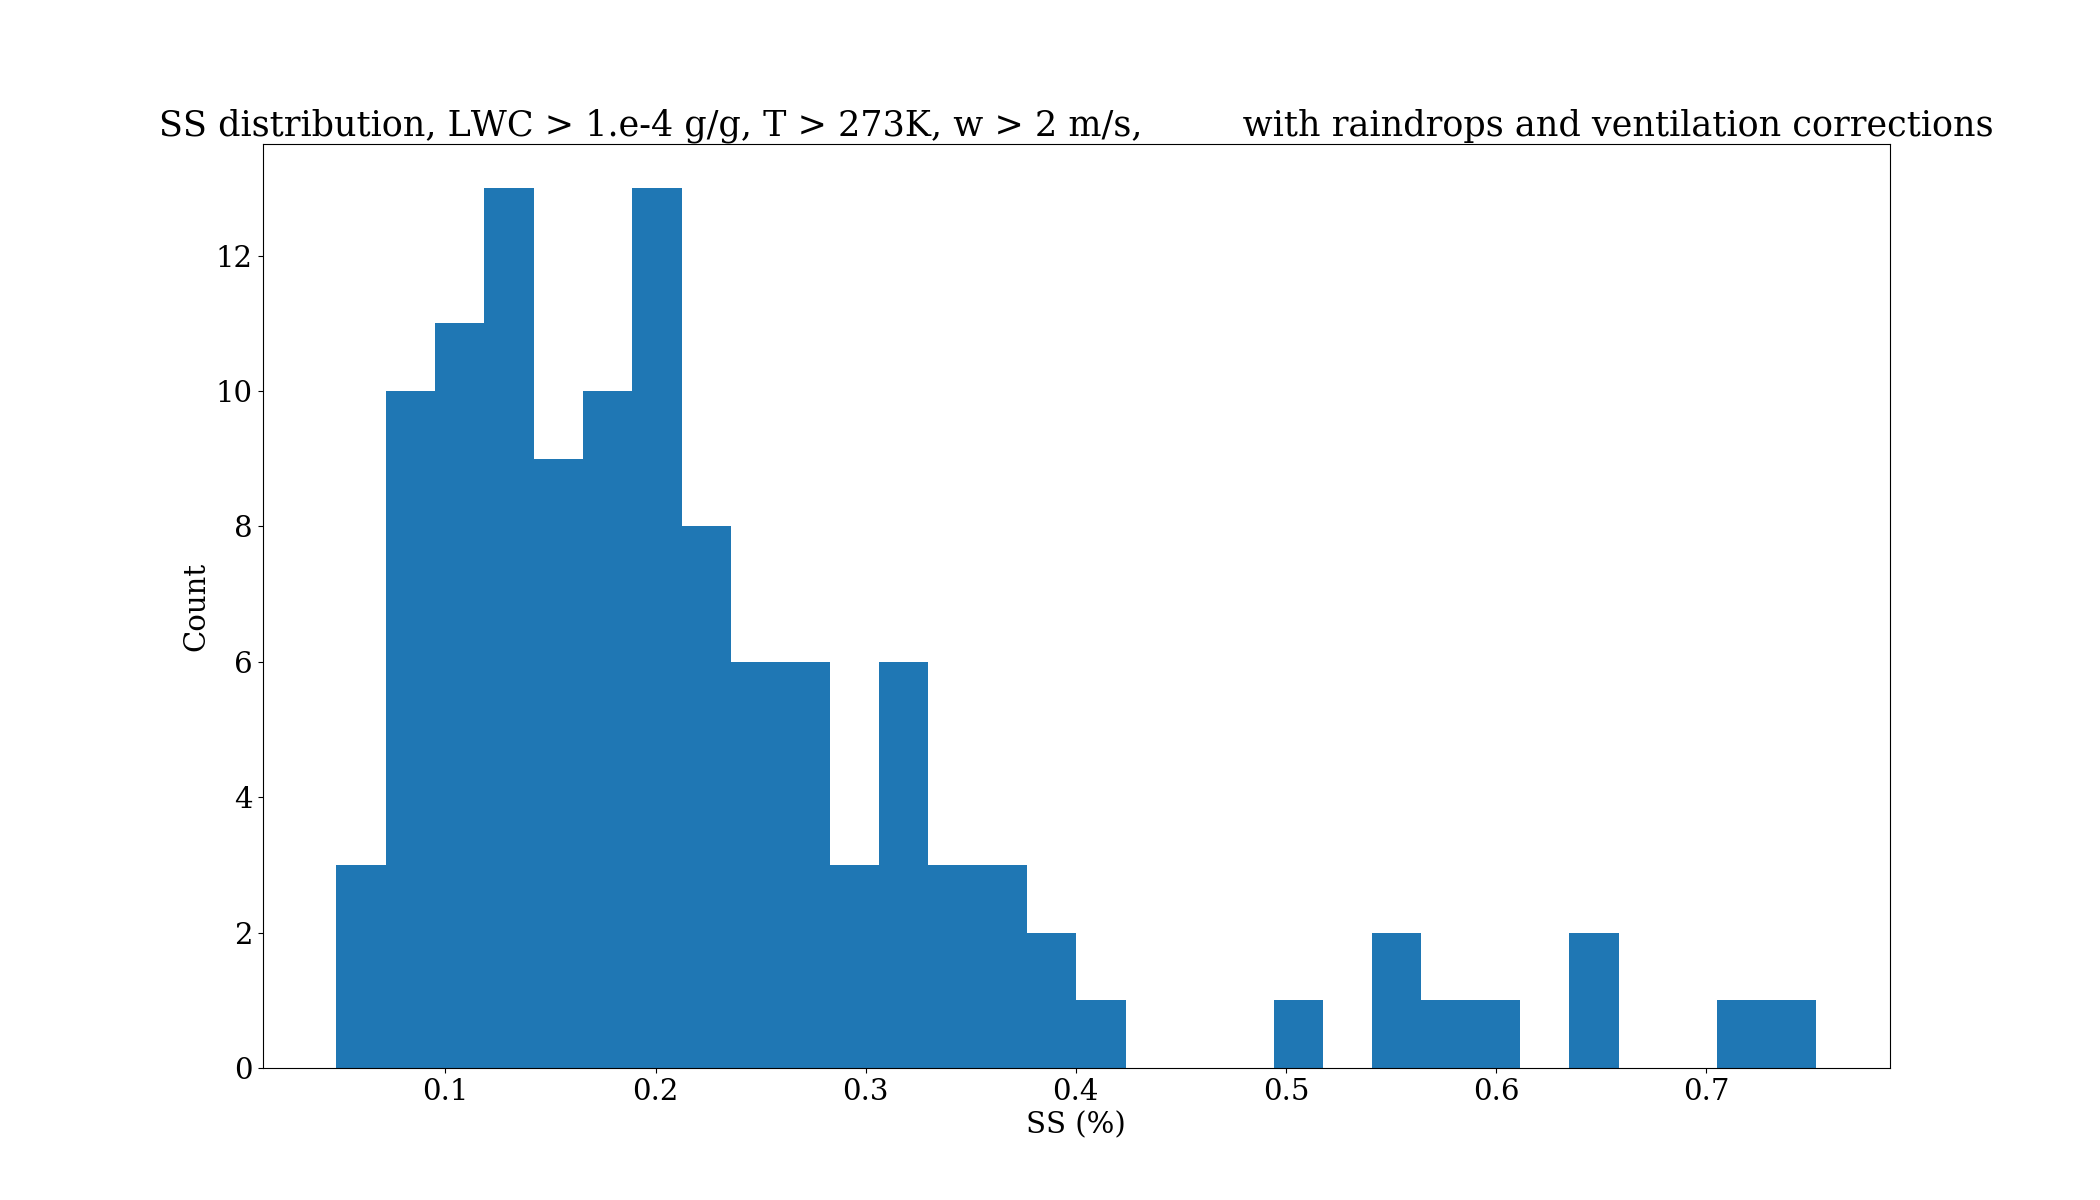
\includegraphics[width=9cm]{halo/v3_ss_with_cip_from_cas_alldates_figure.png}
    \caption{Predicted ($SS_{QSS}$) supersaturation distribution from HALO field campaign (all flight dates). Using filtering criteria outlined in section 2.}
    \label{haloqsshist}
\end{figure}
\begin{figure}[ht]
    \centering
    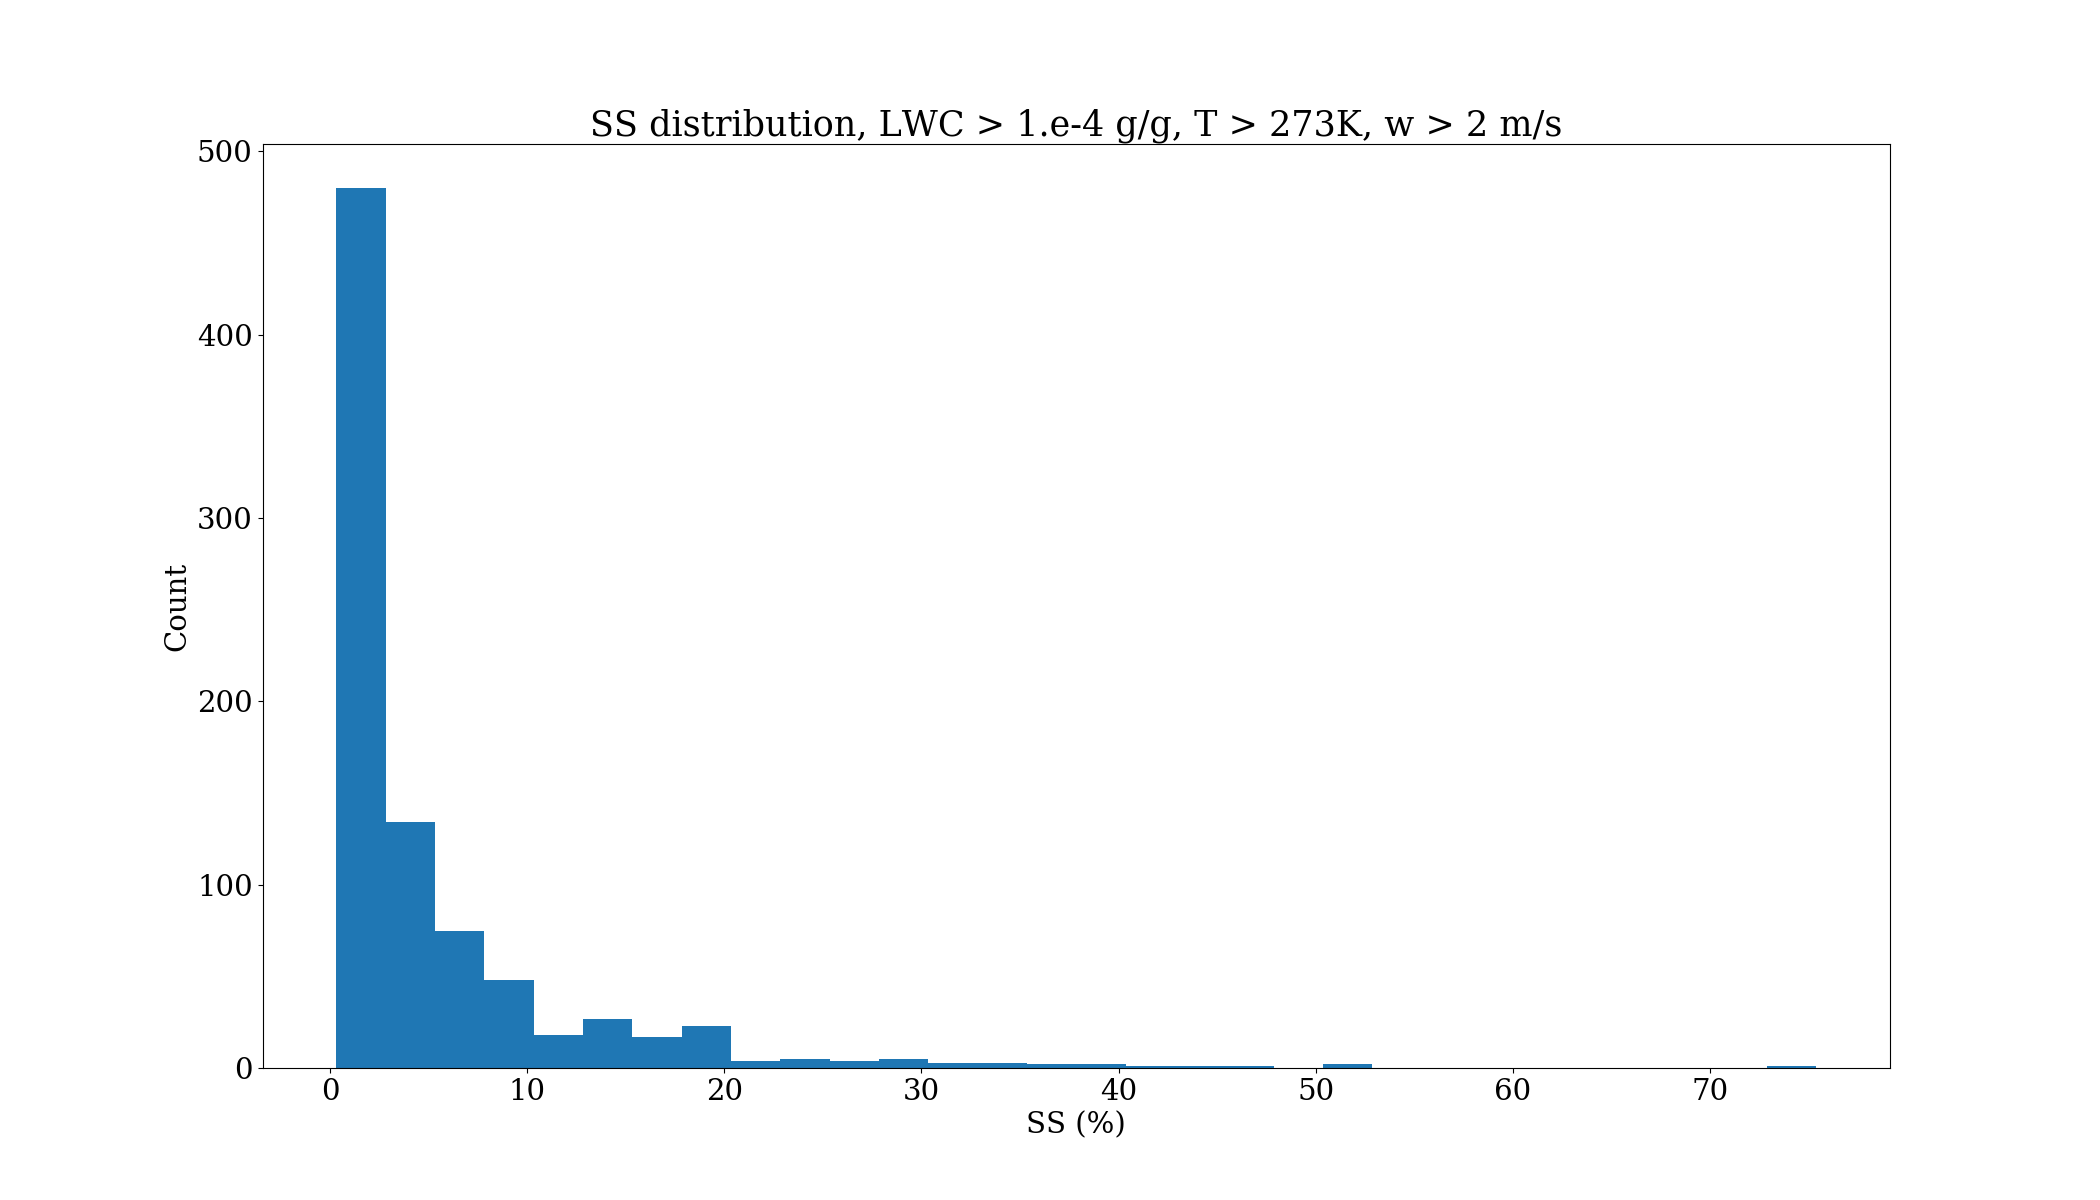
\includegraphics[width=9cm]{caipeex/v1_ss_from_dsd_alldates_figure.png}
    \caption{Predicted ($SS_{QSS}$) supersaturation distribution from CAIPEEX field campaign (all flight dates). Using filtering criteria outlined in section 2, but not including rain drops or ventilation corrections due to lack of data.}
    \label{caipeexqsshist}
\end{figure}
\section{Line of argument}
\subsection{CLAIM}
Figures \ref{haloqsshist} and \ref{caipeexqsshist} demonstrate that we don't observe the same high supersaturations seen in LES simulations (i.e. WRF data) 
\subsection{POSSIBLE COUNTERARGUMENTS}
\begin{enumerate}
	\item Experimentalists just didn't fly through strong enough convective cells / cloudy enough regions (see figs \ref{wrfwhist} and \ref{wrflwchist} which show somewhat broader ranges than we observe from the campaign data).
	\item Experimental sites were too polluted to observe the high supersaturations
	\item Something must be wrong because the CAIPEEX and HALO supersaturation distributions look very different
	\item (more philosophical I guess) If you don't trust WRF to give you realistic supersaturation values then why do you trust it to give you the reasonable regime of validity for the QSS approximation?
\end{enumerate}
\subsection{POSSIBLE COUNTERARGUMENTS TO THE POSSIBLE COUNTERARGUMENTS}
\begin{enumerate}
	\item In fact in the WRF data we don't see a strong correlation (for the data filtered as described above) between $SS_{QSS}$ and...
	\begin{itemize}
		\item LWC (fig \ref{ssqssvslwc})
		\item w (fig \ref{ssqssvsw})
	\end{itemize}
	\item Compare experiment vs simulation for **mystery kernel** integrated over aerosol distribution
	\item \^ ditto but compare CAIPEEX vs HALO
	\item Not sure yet.
\end{enumerate}
\section{Figures to include in supplementary info}
\begin{itemize}
	\item figs \ref{haloqsshist} and \ref{caipeexqsshist} but without lower bin cutoffs
	\item figs \ref{haloqsshist} and \ref{caipeexqsshist} but without corrections from including raindrops / ventilation factors
\end{itemize}
\section{TODO / remaining questions}
\begin{itemize}
	\item error analysis for experimental data
	\item look into commensurate binning in simulation / experiment comparisons?
	\item analytical justification for why actual and QSS supersaturation is still in linear relation
\end{itemize}
This is a reference \cite{Fan2018}.
%\begin{figure}[h]
%    \centering
%    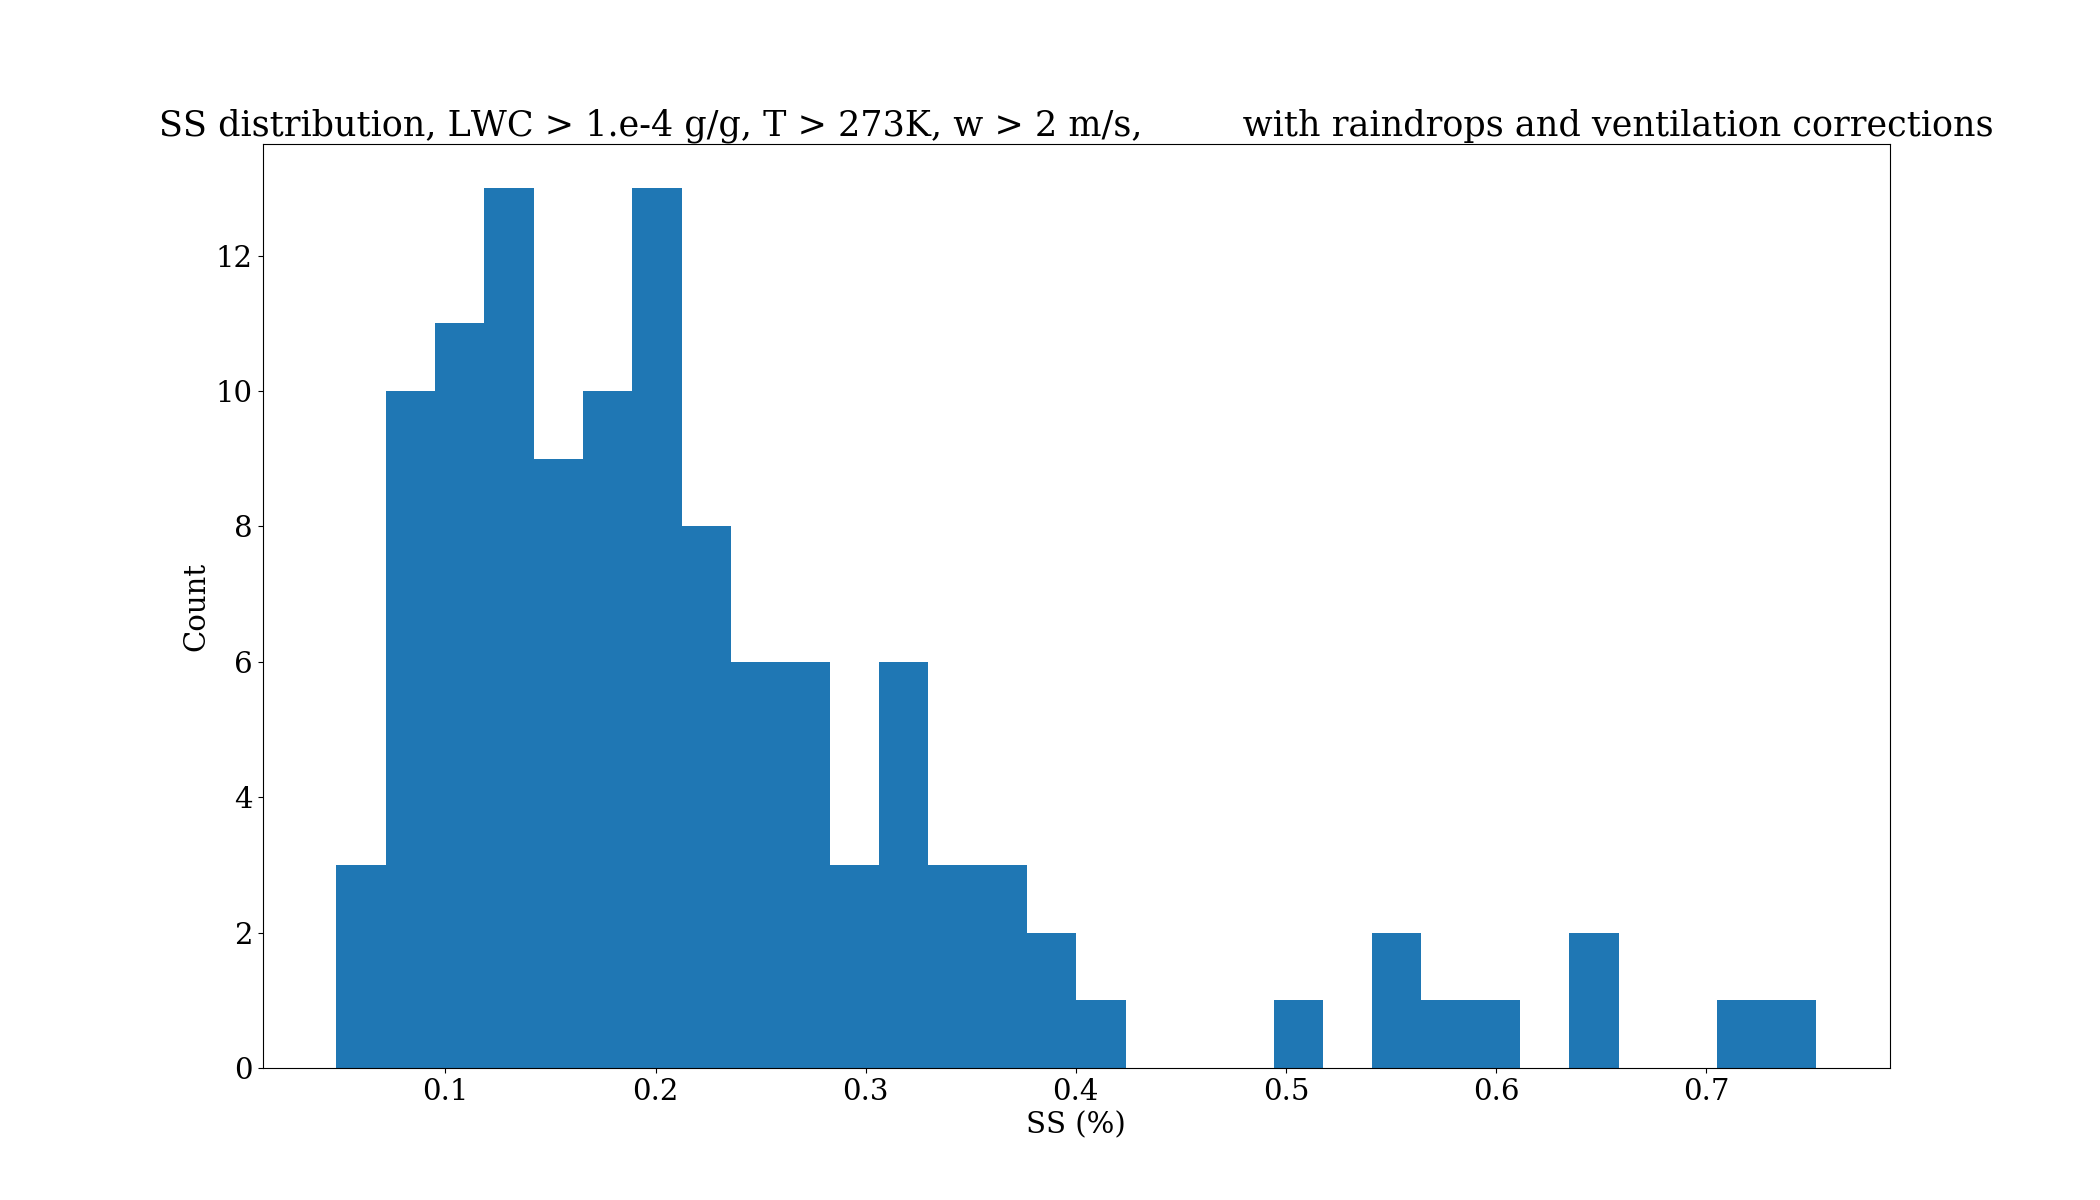
\includegraphics[width=9cm]{halo/v3_ss_with_cip_from_cas_alldates_figure.png}
%    \caption{}
%    \label{fig:fig_label}
%\end{figure}

\bibliography{refs}
\bibliographystyle{ieeetr}
\end{document}
